\documentclass[12pt, letterpaper]{article}     %Tipo de documento
\usepackage[utf8]{inputenc}
\usepackage{graphicx}
\graphicspath{{Images/}}
  \title{Proyecto Final: Bases de Datos}
  \author{Diego Armenta Tezcucano}
	\date{Mayo 22 de 2020}
\begin{document}            %Inicio del documento
	\maketitle
	\textbf{Introduccion}:
	
	\vspace{5mm} %5mm vertical space
	El siguiente proyecto tiene como objetivo la creación de una base de datos para una tienda de abarrotes. A partir de los requerimientos presentados por el cliente se realizo un análisis para poder crear la base que mejor funcionara para el problema en concreto. Se determinó que el objetivo principal era el de realizar ventas y tener registro de lo que éstas involucraban; como el inventario y sus productos; los clientes y proveedores.
	
	\vspace{5mm} %5mm vertical space
	\textbf{Plan de trabajo}:
	
	\vspace{5mm} %5mm vertical space
	Se organizó el plan de trabajo en cuanto a la prioridad de los entregables.
	Los pasos tomados para realizar el proyecto fueron los siguientes:
	
	1.- Creación de diagrama Entidad-Relación.
	
	2.- Creación de Modelo Relacional.
	
	3.- Creación de tablas y normalización.
	
	4.- Programación de base.
	
	5.- Creación de archivos CSV.
	
	6.- Scripts para CSV.
	
	7.- Programación de funciones y triggers de la base.
	
	8.- Revisión del funcionamiento de las funciones.
	
	9.- Diseño de la interfaz web.
	
	10.- Relacionar interfaz con base de datos.
	
	11.- Documentación.
	
	\vspace{15mm} %5mm vertical space
	\textbf{Diseño}:
	
	\vspace{5mm} %5mm vertical space
	1.- Diagrama Entidad-Relación:
	
	\vspace{5mm} %5mm vertical space
	%la
	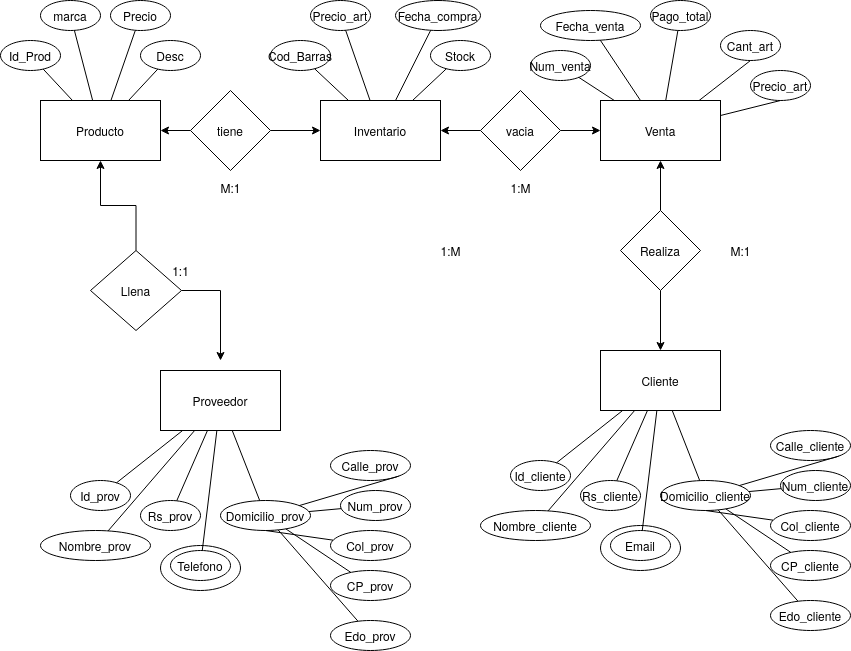
\includegraphics[scale=0.4]{DiagramaER}

	Una de las primeras propuestas que se tuvo del diagrama fue la de unir proveedor, producto y venta mediante inventario. Al principio esto parecía tener muchas ventajas ya que las entidades más importantes estarían unidas mediante el código de barras, además parecía tener sentido que un proveedor llenara el inventario, el inventario administrara los productos y las ventas. Sin embargo, esto hacia que la llave cod\_barras se propagara hacia proveedor y en consecuencia hacia telefono ya que es un atributo multivaluado, por lo que se notó que esta configuración propagaba datos donde no se necesitaban.
	
	La propuesta decisiva relaciona al proveedor con el producto, y el inventario conecta las ventas con el producto.	
	
	Se realizo el diagrama tomando en cuenta que si se relacionaba un inventario con muchos productos y muchas ventas se tendría la llave primaria del mismo (cod\_barras) al alcance de los entidades más importantes, lo que permitiría relacionar facilmente producto con venta e inventario con cualquiera de las dos.
	
	Por otro lado, la idea original entre la relación de producto y proveedor era que un proveedor pudiese surtir varios productos. Al análizar el problema se llego a la conclusión de que utilizando una relación uno a uno y pasando la clave del proveedor al producto generaba la misma funcionalidad, pero eliminaba de la llave primaria de producto el id\_proveedor. Lo que soluciono conflictos a la hora de normalizar ya que no había necesidad de que los detalles del producto dependieran del id del proveedor.
	\vspace{5mm} 
	
	2.- Modelo Relacional.
	
	\vspace{5mm} %5mm vertical space
	\begin{center}
	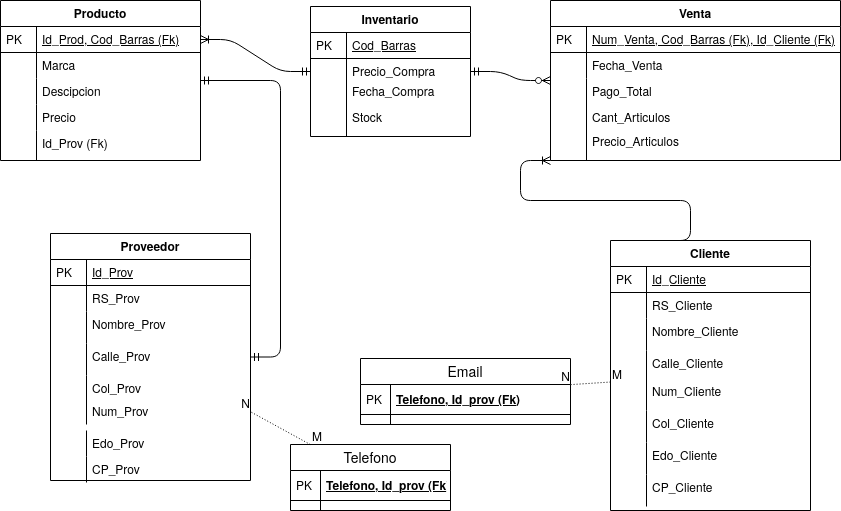
\includegraphics[scale=0.4]{ModeloRelacional}
	\end{center}
	
	\begin{center}
	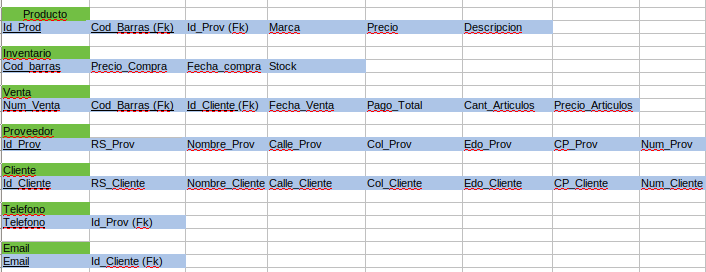
\includegraphics[scale=0.45]{tabla}
	\end{center}	
	
	\pagebreak
	3.- Normalización.
	\vspace{5mm} %5mm vertical space
	Con las tablas siguientes se comenzó la normalización:
	
	\begin{center}
   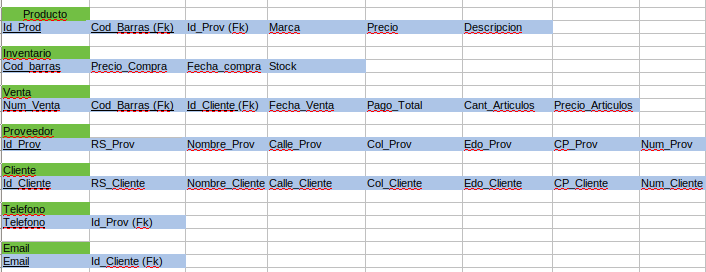
\includegraphics[scale=0.45]{tabla}
	\end{center}
	
	Primera Forma Normal:
	
	Se separarón los grupos de repetición de la tabla Proveedor, estos incluian el CP, el Num\_Prov (numero de vivienda) y el Edo. Los atributos anteriores se pasaron a otra tabla, aquí al hacer lo mismo con la tabla cliente se notó que no había la necesidad de tener codigos postales separados para cliente y proveedor por lo que se utilizó una sola tabla para ambos.
	
	También se separaron los grupos de repetición en la tabla Venta, que inlcuían el código de barras, la cantidad de articulos y el precio de los mismos. Esta información de pasó a otra tabla (venta\_detalles) de manera que los datos generales de la venta estuviesen en una, y los detalles de la venta en otra.
	
	\vspace{5mm} %5mm vertical space
	\begin{center}
   	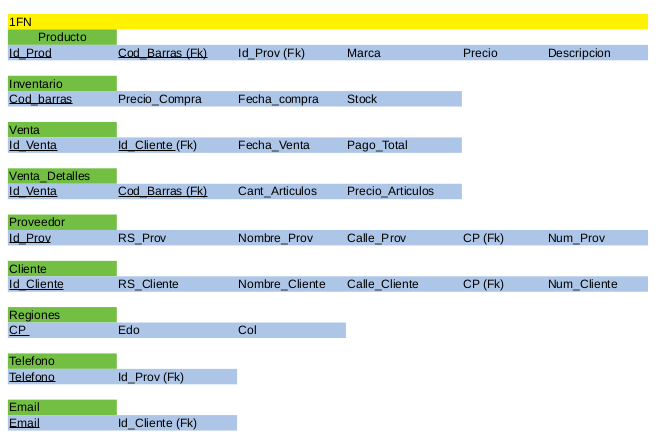
\includegraphics[scale=0.45]{tabla1N}
	\end{center}
	
	Segunda Forma Normal:
	
	Para esta etapa de nomalización de identificó que la tabla producto contenía para todos los atributos dependencias parciales en Id\_prod y Cod\_Barras por lo que estos dos valores se pusieron en una tabla aparte y se dejo la tabla restante con Cod\_Barras. La necesidad de un Id\_prod en este momento podría parecer innecesaria. Pero muchas veces los codigos de barras de los productos no se encuentran, además de que son largos. Por lo que tener un Id\_para el producto es necesario además de que originalmente es la llave primaria del producto.

	\vspace{5mm} %5mm vertical space
	\begin{center}
   	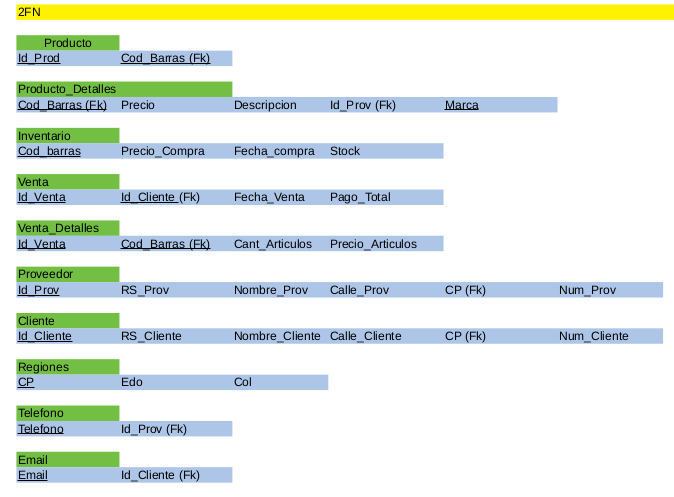
\includegraphics[scale=0.45]{tabla2N}
	\end{center}	
	
	Tercera Forma Normal:
	
	Para la tercera forma normal se determino que en la tabla Producto\_Detalles existía una relación transitiva del codigo de barras al id del proveedor, y de éste a la marca del producto, ya que si los proveedores son oficiales no venderan productos que no sean de su compañia, asi que se paso Id\_prov y marca  a otra tabla.
	
	\begin{center}
   	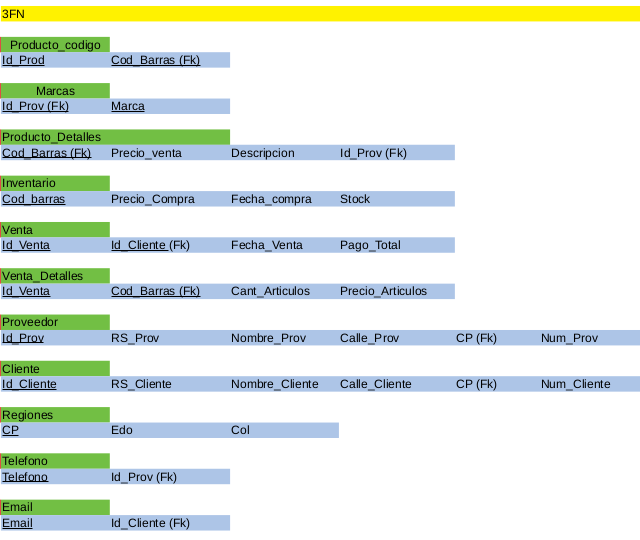
\includegraphics[scale=0.4]{tabla3N}
	\end{center}	
	
	\textbf{Implementación}:
		\vspace{5mm} %5mm vertical space

	
	En la siguiente sección se listan unicamente las funciones, procedimientos y triggers que permiten realizar las actividades solicitadas en los procedimientos.
	
	\vspace{5mm} %5mm vertical space
	Requerimiento 1:

	La siguiente función permite el cálculo de la utlidad a partir del precio de compra en el inventario y el precio de venta en el producto. El parámetro enviado es el codigo de barras del producto. En este caso los códigos de barra son muy simples para fines demostrativos.
	
		
	\begin{center}
   	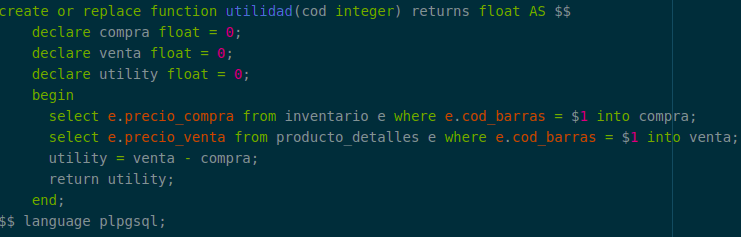
\includegraphics[scale=0.50]{req1}
	\end{center}
	
	\pagebreak
	Requerimiento 2:

	El primer punto del requerimiento que se trató fue el de darle numeración a las ventas de manera que el siguiente trigger forza que cada vez que se inserte una nueva venta se guarde como id, en el formato "Vent\_000" de manera secuencial.
	
		
	\begin{center}
   	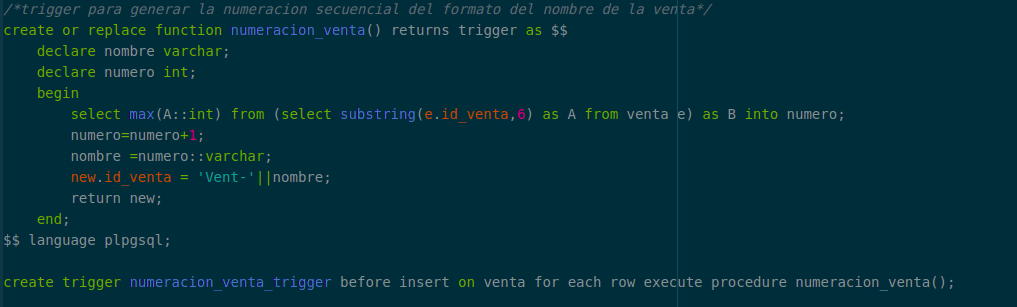
\includegraphics[scale=0.40]{req22}
	\end{center}
	
	De manera similar se realizó un trigger para tener los clientes de manera secuencial, ésto no se pidió explicitamente pero ayudó a la hora de realizar el agregado de la venta. Considerando que no todos los clientes que compraran iban a querer registrarse.
	
	\begin{center}
   	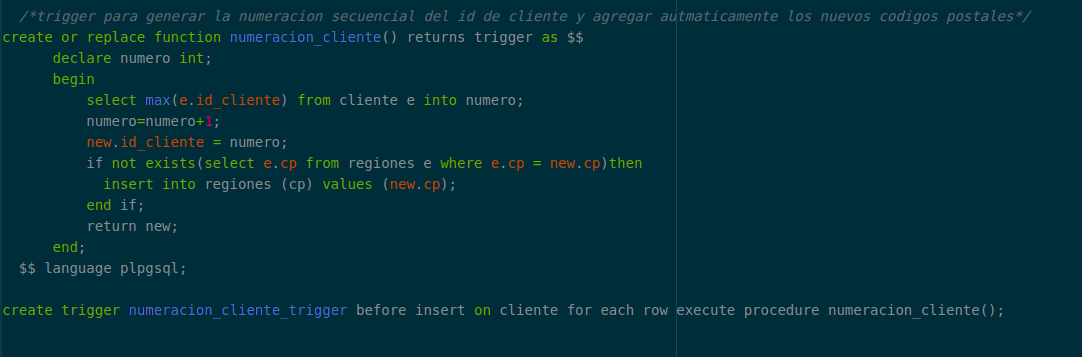
\includegraphics[scale=0.40]{req23}
	\end{center}
	
	Lo siguiente fue crear una funcion para facilitar el agregado de una venta, se crearon dos funciones: una para crear una venta hecha por un cliente registrado y otra para clientes que no quisieran darse de alta. La segunda crea un cliente sin registro y lo asigna a la venta.
	
	\begin{center}
   	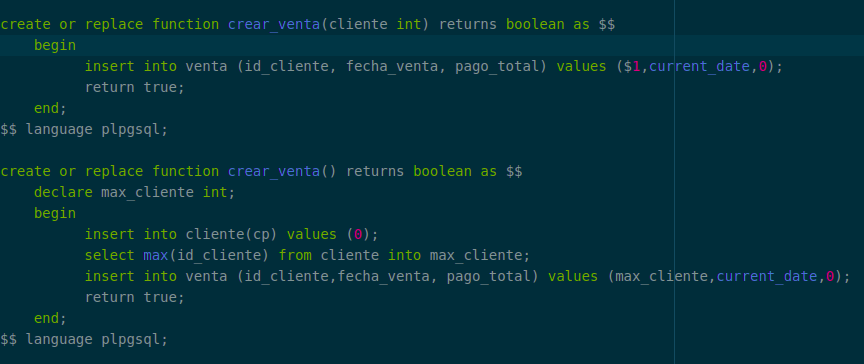
\includegraphics[scale=0.40]{req2}
	\end{center}
	
	La siguiente parte es un trigger que verifica que los productos cumplan los requisitos de stock, si no hay stock no permite la inserción y envia una alerta que diga que el stock es insuficiente. Tambien decrementa elstock al completar la venta.
	
	Aqui se incluyeron dos funciones más para la generación de información, el calculo del subtotal por producto y el calculo del total de la venta.	
	
	
	\begin{center}
   	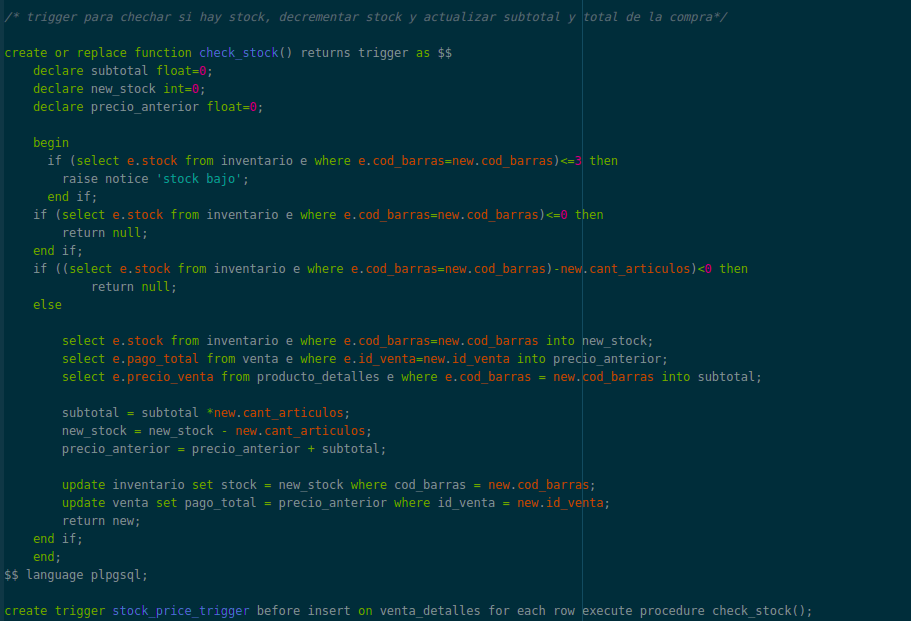
\includegraphics[scale=0.40]{req26}
	\end{center}
	
Por último se agrego una funcion para facilitar la inserción de un producto en la venta así como los datos de subtotal calculados anteriormente y la actualización del pago total de la venta a medida que entran productos.	

	
	\begin{center}
   	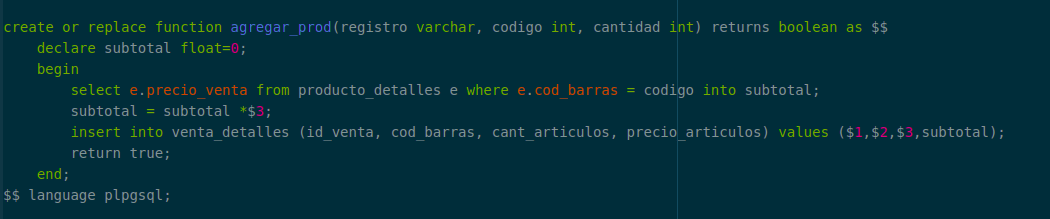
\includegraphics[scale=0.40]{req24}
	\end{center}
	
	Requerimiento 3:
	
	Para este requerimiento se crearon dos funciones que regresen la cantidad de productos vendidos por producto, una lo realiza recibiendo como parámetro una fecha específica, la otra devuelve los resultados en un periodo delimitado por dos fechas.
	
	
	\begin{center}
   	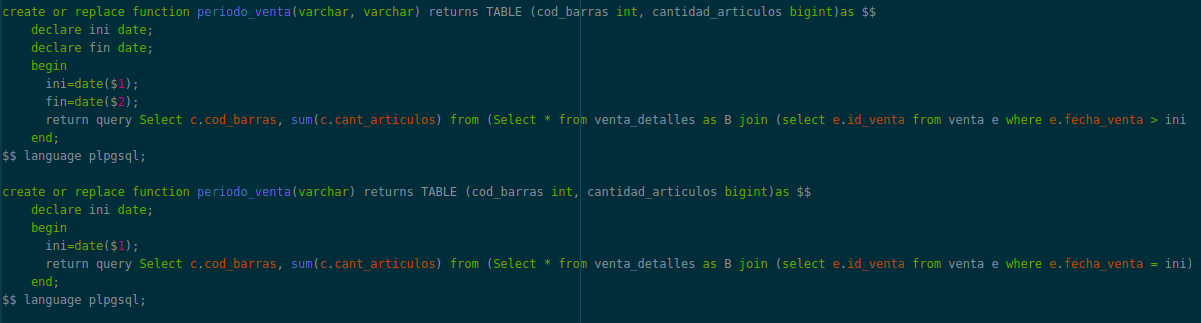
\includegraphics[scale=0.35]{req3}
	\end{center}
	
	Requerimientos 4:
	
	Para el requerimiento 4 se creo la funcion productos\_escasos() que permite obtener sin parámetros todos los productos que tengan menos de 3 en stock.
	
			\vspace{5mm} %5mm vertical space

	Requerimiento 5:
	
			\vspace{5mm} %5mm vertical space

	Se realizó una función que recolecte toda la informacion de las diferentes tablas (inventario, venta y productos) que pueda ser utilizada en una factura. La funcion se llama info\_factura().
	
			\vspace{5mm} %5mm vertical space

	Requerimiento 6:
	
	Se implemento un índice en el codigo de barras considerando que la tabla de productos es la más grande y que el atributo es compartido en multiples tablas.
	
		
	\begin{center}
   	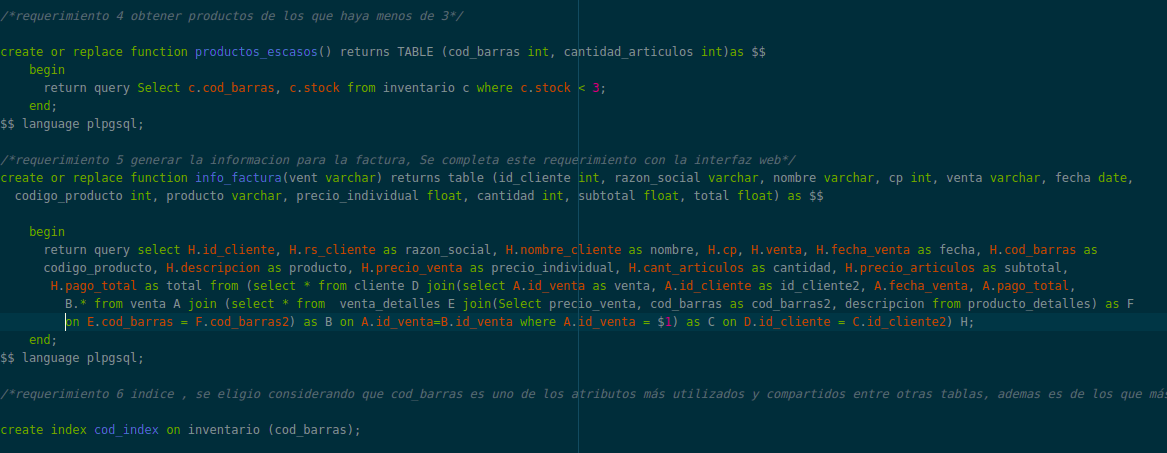
\includegraphics[scale=0.35]{req456}
	\end{center}
	
		\vspace{5mm} %5mm vertical space

		\textbf{Pruebas:}
		\vspace{5mm} %5mm vertical space

		
		Requisito 1.-
		
		La funcion utlidad() regresa la ganancia de un producto dado su codigo de barras. En este caso los codigos de barras son simples para fines de ejemplificación.
		
		\begin{center}
 	  	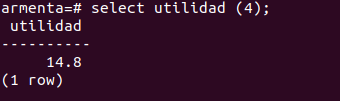
\includegraphics[scale=0.75]{utlidad_function}
		\end{center}
		
		Requisito 2.-
		
		Con las funciones descritas para el requerimiento 2 en la etapa de implementación, se realizó la interfaz web que hace uso de las mismas para la inserción de una venta.
		
		Este requerimiento se complementa con la interfaz web.
		
		
		Ejemplo desde sql:
		
		Se crea una venta nueva:
		
				
		
		\begin{center}
 	  	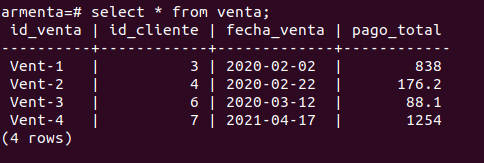
\includegraphics[scale=0.5]{venta_prev}
		\end{center}
		
		\begin{center}
 	  	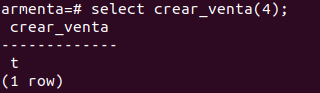
\includegraphics[scale=0.5]{crear_venta}
		\end{center}
		
		En los detalles siguientes se muestra la venta y como no hay ningun producto registrado en ella.		
		
		\begin{center}
 	  	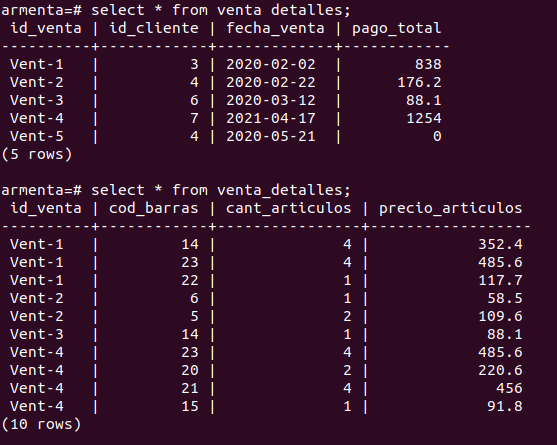
\includegraphics[scale=0.5]{venta_after}
		\end{center}
		
		Se llama el registro del inventario antes de agregar el producto, fije su atencion en el producto con codigo de barras 23.	
		
		\begin{center}
 	  	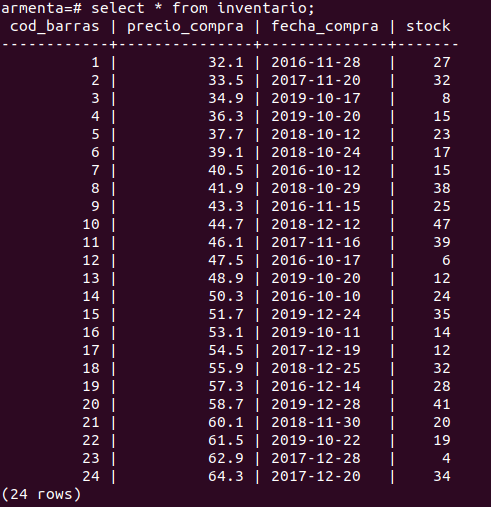
\includegraphics[scale=0.5]{inventario_prev}
		\end{center}
	
		Se agrega el producto.
						
		\begin{center}
 	  	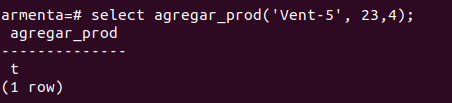
\includegraphics[scale=0.7]{agregar_prod}
		\end{center}
				
		Ahora el trigger se llama automaticmante y el stock de ese producto baja.		
		
		\begin{center}
 	  	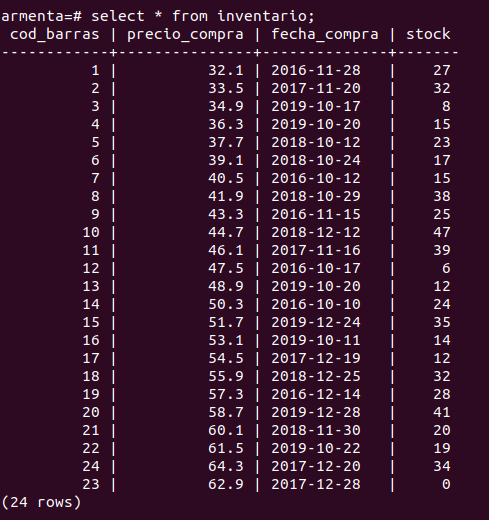
\includegraphics[scale=0.5]{trigger_disminuir_stock}
		\end{center}
		
		Si se intenta agregar la cantidad de un producto que supere el stock disponible, esta no se agregara a la venta y enviara una alerta. Preste atencion al producto 3
		
		\begin{center}
 	  	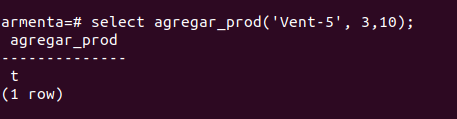
\includegraphics[scale=0.5]{agregar_prod_insuficiente}
		\end{center}
		
		Efectivamente el stock permanece sin cambio.
		
		\begin{center}
 	  	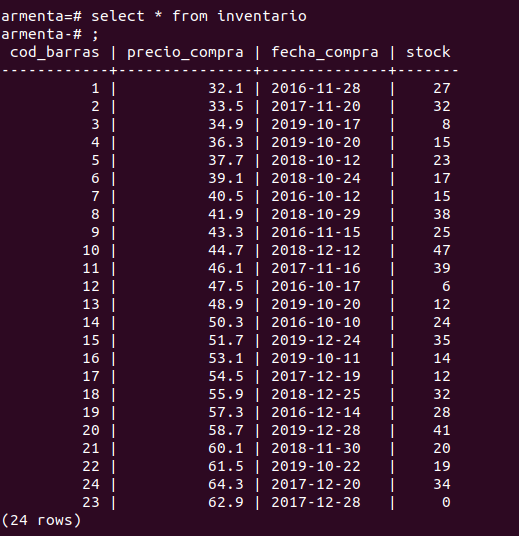
\includegraphics[scale=0.5]{inventario_stock_insuficiente}
		\end{center}
		
		Los detalles de la venta (Vent\_5) muestran como sólo se agrego el producto en existencia a la misma.
		
		\begin{center}
 	  	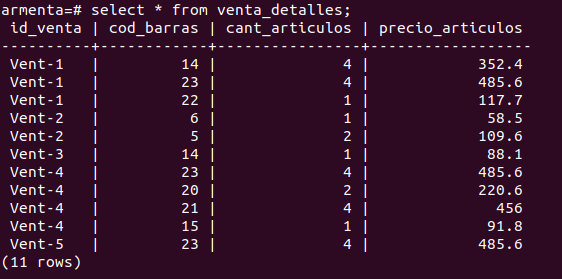
\includegraphics[scale=0.5]{venta_detalles_after_agregar}
		\end{center}
		\pagebreak
		Requerimiento 3:
		
		Se muestran los productos vendidos en una fecha y en un periodo entre fechas.
		
			\begin{center}
 		  	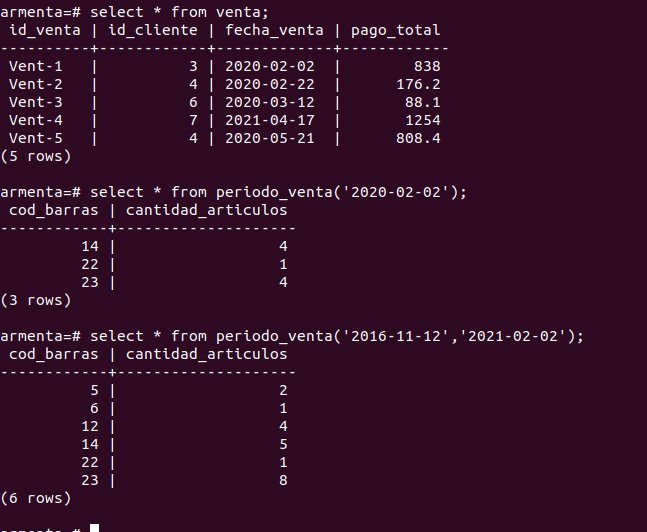
\includegraphics[scale=0.5]{3_periodo_venta_simple}
			\end{center}
				
		
				\vspace{5mm} %5mm vertical space

		Requerimiento 4:
		
		Se muestran los productos donde hay stock bajo (menor a 3)		
		
		\begin{center}
 	  	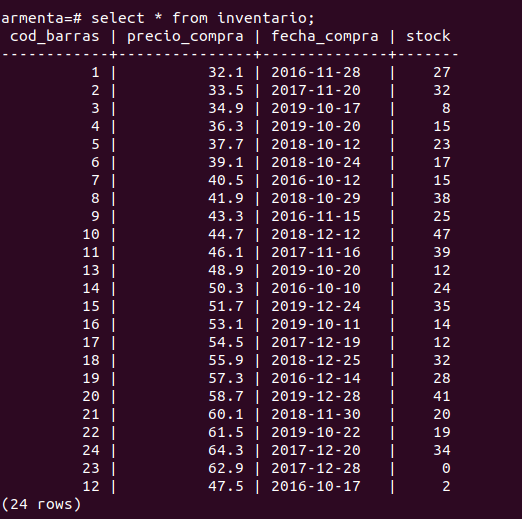
\includegraphics[scale=0.5]{4_inventario_prod_escasos}
		\end{center}
		
		\begin{center}
 	  	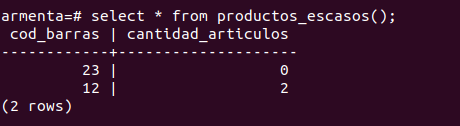
\includegraphics[scale=0.5]{4_prod_escasos}
		\end{center}
		
		\vspace{5mm} %5mm vertical space

		Requerimiento 5:
		
		Se muestran la informacion necesaria para una factura, este requerimiento se complementa con la interfaz web.
		
		\begin{center}
 	  	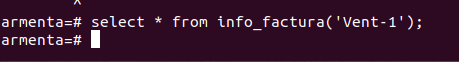
\includegraphics[scale=0.5]{5_factura_1}
		\end{center}
		
		\begin{center}
 	  	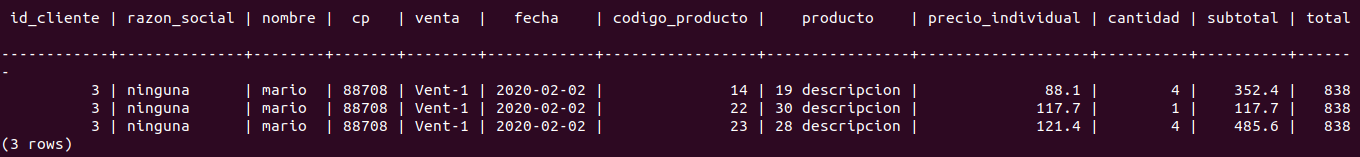
\includegraphics[scale=0.35]{5_factura_2}
		\end{center}
			
		
		\vspace{5mm} %5mm vertical space

		\textbf{Pruebas en interfaz web:}
		\vspace{5mm} %5mm vertical space
		
		Pruebas para la insercion de cliente:

		Se verifican los clientes antes de comenzar el proceso:
		
		\begin{center}
 	  	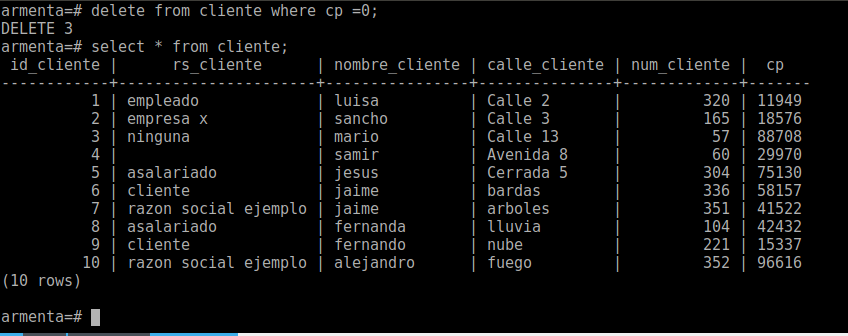
\includegraphics[scale=0.5]{web_cliente_prev}
		\end{center}
		
		Se realiza el proceso de agregar cliente.
				
		
		\begin{center}
 	  	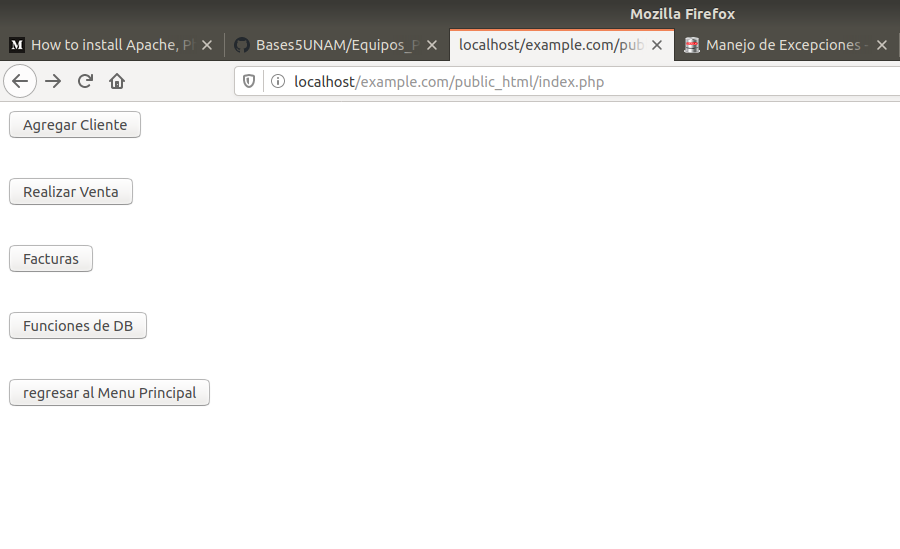
\includegraphics[scale=0.5]{web_menu}
		\end{center}
		
		\begin{center}
 	  	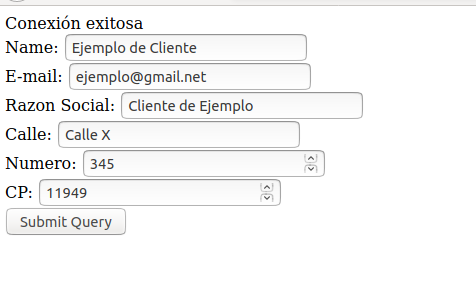
\includegraphics[scale=0.5]{web_cliente_datos}
		\end{center}
		
		Se verifica en la base que se haya agregado el cliente:
		
		\begin{center}
 	  	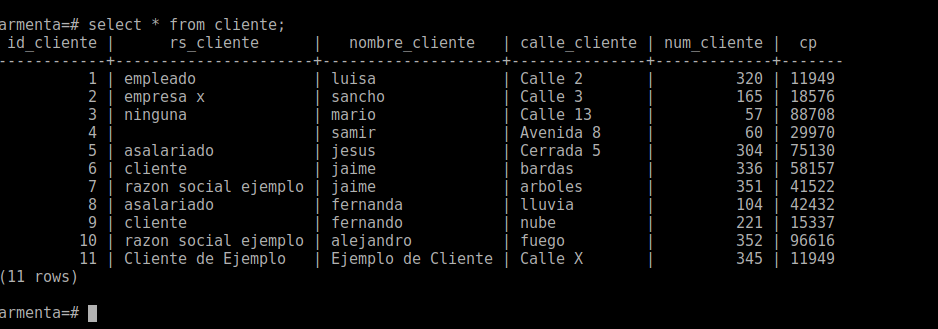
\includegraphics[scale=0.5]{web_cliente_after}
		\end{center}
		
		Prueba para la venta y factura:
		
		Se verifican los datos de ventas antes de iniciar el proceso:
				
		
		\begin{center}
 	  	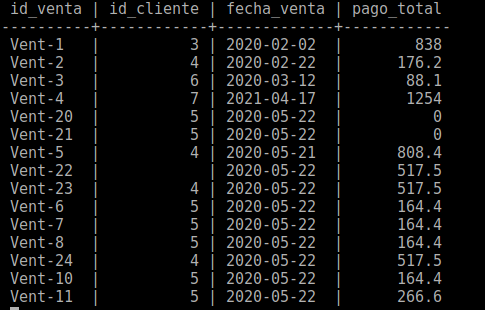
\includegraphics[scale=0.5]{web_venta_prev_1}
		\end{center}
		
		\begin{center}
 	  	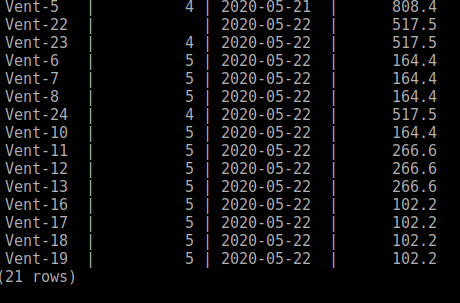
\includegraphics[scale=0.5]{web_venta_prev_2}
		\end{center}
		
		Se realiza el agregado desde la interfaz.
		
		\begin{center}
 	  	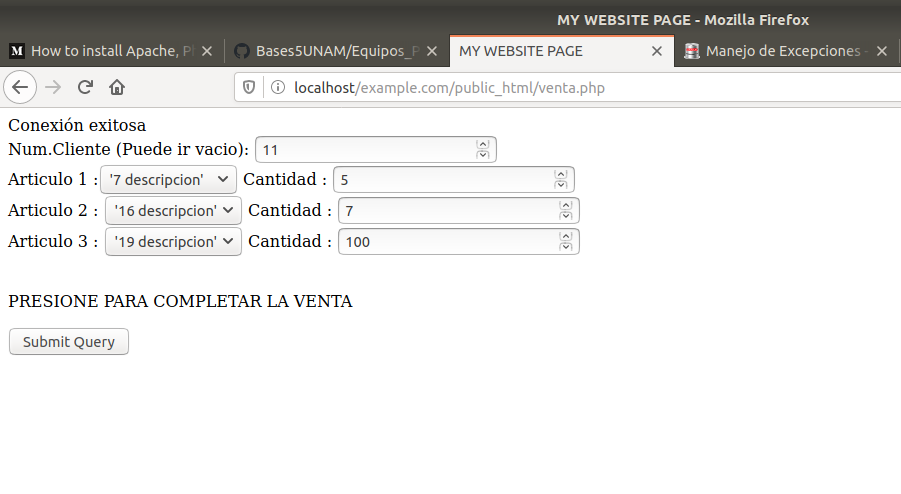
\includegraphics[scale=0.5]{web_venta_agregar}
		\end{center}
		
		La interfaz nos muestra que se completó la venta y muestra los datos de la factura haciendo uso de las funciones implementadas en la base.
		
		No se agregan los productos para los que no haya stock suficiente, en la parte hay un aviso de stock insuficiente para un producto, pero si se agregan los productos que existen.		
				
		\begin{center}
 	  	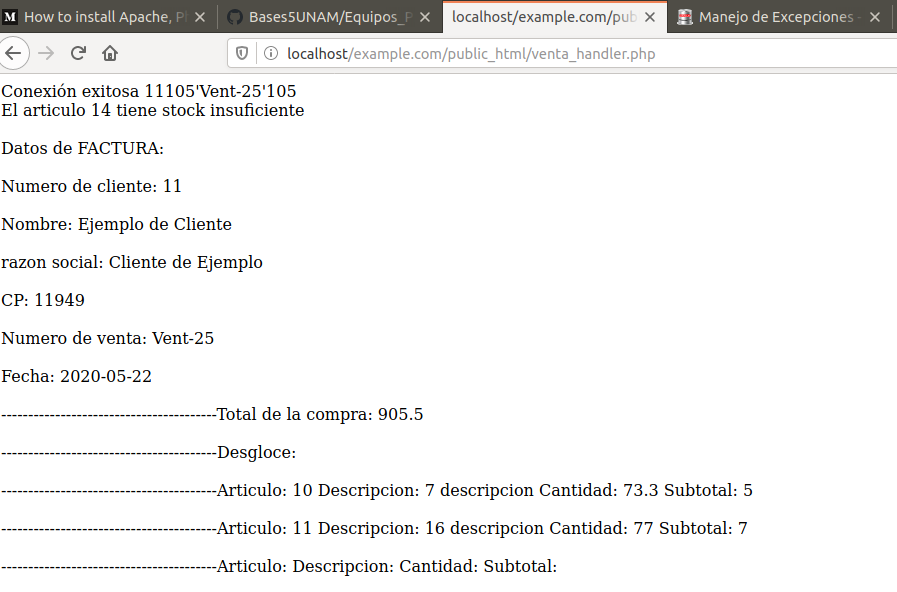
\includegraphics[scale=0.5]{web_venta_res}
		\end{center}		
		
		Se muestra en la base que la venta se agregó, asi como los detalles de cada producto en la misma.		
		
		\begin{center}
 	  	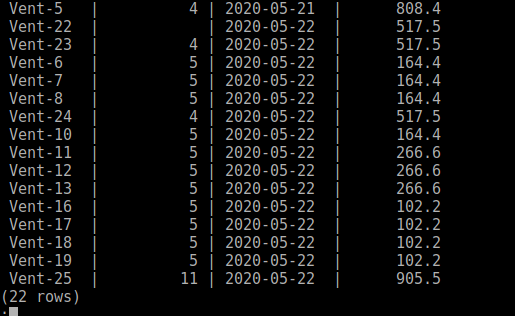
\includegraphics[scale=0.5]{web_venta_after}
		\end{center}
		
		\begin{center}
 	  	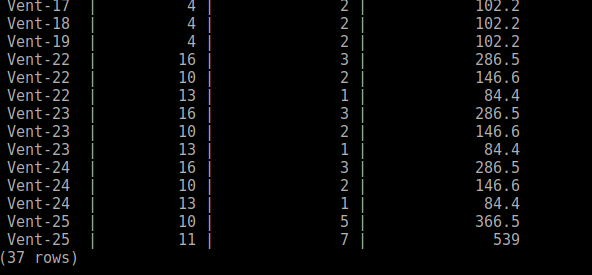
\includegraphics[scale=0.5]{web_venta_detalles_after}
		\end{center}
		
		\vspace{5mm} %5mm vertical space
		\textbf{Conclusiones}:
		\vspace{5mm} %5mm vertical space
		
		Este proyecto requirio una cantidad fuerte de esfuerzo y dedicación, cada seccion del mismo no fué trivial y realizarla exigía prestar atención a lo que se estaba haciendo, así como pensar cual era la mejor solución al problema.
		
		La etapa de diseño me permitió ver lo importante que es el estructurar bien la base desde el inicio, ya que si no se hace de forma correcta a lo largo de las demás fases irán surgiendo problemas que será dificil arreglar y requerirá soluciones menos elegantes. Al inicio del documento se menciono que existian diferentes propuestas de resolución, al intentar trabajar con estas propuestas se generaron el tipo de problemas mencionados anteriormente, por lo que la propuesta seleccionada se hizo en base no solo al análisis de la misma sino también al verificar que implementandola se trabajaría en las demás fases de una manera más fluida.
		
		La etapa de nomalización de igual manera represento un ejercicio de análisis para determinar el propósito del proceso. De igual manera que en la fase anterior, el intentar utilizar propuestas descartadas para la nomalización generaba tablas que poco ayudaban al entendimiento de los datos y a la resolución del problema. Las tablas generadas a partir de las propuestas descartadas relacionaban datos en sitios que no los necesitaban o donde incluso eran más un impedimento para manejar la información.
		
		La etapa de implementación fue la que personalmente más disfruté pues me permitio hacer uso de los conocimientos clásicos de programación para gestionar características de la base, en esta fase fue que me dí cuenta de cuál poderosas son las bases de datos y del porque la importancia de la programación dentro de la base. La programación PL/SQL permite crear límites dentro de la base en cuanto a seguridad, pero también permite extenderla a manera que la gestión de datos sea mucho más sencilla e incluso procese información acerca de quien maneja la base.
		
		En general creo que fue un ejercicio muy interesante que permitio poner a prueba lo aprendido a lo largo del curso. Fue una oportuinidad de adentrarme en un campo que conocía de una manera muy superficial y que ahora ha generado gran interes en mi.		
		
		



\end{document}               %Final del documento
 